\chapter{Numerical Simulation of Heat Transfer} % Main chapter title

\label{Chapter4}

\section{OpenFOAM: chtMultiphaseInterFOAM. Conjugate Heat Transfer}
\setlength{\parindent}{0.5cm} The last objective of this thesis is to extend the multiphase solver of the previous section so it can account for multiregion purposes. To do so, a new solver derived from the concept of an existing multiregion solver is implemented. 

\noindent The existing solver, \textit{chtMultiRegionFoam} is developed on the basis that the fluid it solves undergoes the compressible Navier-Stokes equations with buoyancy forces and the energy equation per unit mass with gravity terms as follows:
\subsubsection*{Continuity Equation}
The continuity equation reads as:
\begin{equation}
	\frac{\partial \rho}{\partial t}+\nabla \cdot(\rho \boldsymbol{u})=0
	\label{4.1}
\end{equation}
\subsubsection*{Momentum Equation}
The momentum conservation equation yields as:
\begin{equation}
	\begin{aligned}
		&\frac{\partial \rho \boldsymbol{u}}{\partial t}+\nabla \cdot(\rho \boldsymbol{u} \otimes \boldsymbol{u})=\\
		&-\nabla p_{\mathrm{rgh}}+\nabla \cdot\left[\mu\left\{\nabla \otimes \boldsymbol{u}+(\nabla \otimes \boldsymbol{u})^{\mathrm{T}}\right\}\right]
		-\nabla\left(\frac{2}{3} \mu \nabla \cdot \boldsymbol{u}\right)-\boldsymbol{g} \cdot \boldsymbol{x} \nabla \rho
	\end{aligned}
	\centering
	\label{4.2}
\end{equation}
\subsubsection*{Energy Equation}
The energy equation as listed in the native solver is:
\begin{equation}
	\frac{\partial \rho h}{\partial t}+\nabla \cdot(\rho \boldsymbol{u} h)+\nabla \cdot(\rho \boldsymbol{u} K)=\nabla \cdot\left(\frac{\lambda}{c_{p}} \nabla h\right)+\rho \boldsymbol{u} \cdot \boldsymbol{g}
	\label{4.3}
\end{equation}
where \textit{\textbf{u}} is the velocity vector, \textit{h} is the enthalpy, \textit{K = 0.5*\textbf{u $\cdot$ u}} is the kinetic energy per unit mass, \textit{$p_{rgh}=p-\rho\textbf{g}\cdot\textbf{x}$} the modified pressure so that the momentum equation accounts for the buoyancy terms, and the remaining thermophysical properties, $\mu$, $\lambda$, $C_p$ being the kinematic viscosity, the thermal conductivity and the specific heat accordingly. The energy equation does not include radiation, heat generation term and chemical reaction.

Therefore, the challenge of this part is to couple the multiphase solver (\textit{IcoReactingMultiPhaseInterFoam}) that allows for the solving of a fluid undergoing phase-change with a solid region.  
\subsection{Case description}

\setlength{\parindent}{0.5cm} Within this new case, a mesh for the solid region is required. To do so, a second structured mesh region is implemented within the framework of a provided script which builts cylindrical computational meshes in OpenFOAM format. The script is attached in Appendix \ref{AppendixB}.
\begin{figure}[h!]
	\centering
	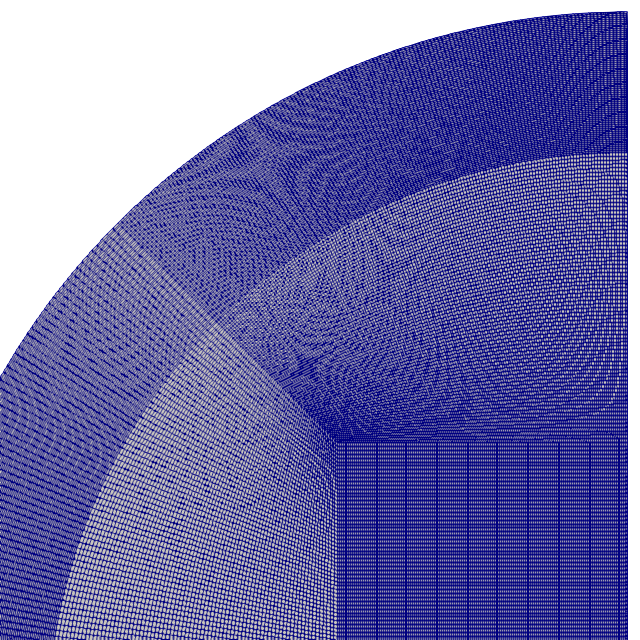
\includegraphics[width=0.6\linewidth]{mesh_CHT.png}	
	\label{4.1fig}
	\caption{Computational mesh for the conjugate heat transfer case.}
\end{figure} 
\newline
In the image shown above, a structured mesh of 731734 nodes is generated.
\subsection{Hypotheses And Assumptions}
\textbf{Heat transfer:} Conductive heat transfer is transferred throughout an isotropic material and convective heat transfer is arisen within the fluid region. 

\textbf{Laminar regime:} The Reynolds number, computed from the maximum velocity is not high enough to consider turbulent effects. 

In the current case-scenario, a Prandtl close to 7. The values used for the laminar Prandtl number calculation are: $\mu = 0.001003 Kg.m^{-1}.s^{-1}$, $\lambda = 0.6 W.m^{-1}.K^{-1}$ and $C_{p}=4182 J.Kg.K^{-1}$.

\textbf{Newtonian fluid:} The viscosity of the fluid is assumed to be constant.
As per the solidification cases, the treatment of the thermophysical properties is performed in a similar manner.

\subsection{Governing Equations of the Fluid Region}
\subsubsection*{Momentum equation}

\setlength{\parindent}{0.5cm} The momentum equation is recalled here in terms of viscous stress tensor. The surface tension forces as the body forces and the Darcy term is added in the momentum equation as shown below.
\begin{equation}
	\label{4.4}
	\begin{aligned}
	&\frac{\partial\left(\rho {u}_{i}\right)}{\partial t}+\frac{\partial\left(\rho {u}_{i} {u}_{j}\right)}{\partial x_{j}} \\
	&\quad=-\alpha_{i} \nabla p+\nabla \cdot \tau +F_{\sigma i}+S_{u_{i}}+S_{b}
	\end{aligned}
\end{equation}
\subsubsection*{Energy equation}

\setlength{\parindent}{0.5cm} The energy equation is also described here in terms of temperature and specific heat. Moreover, as for in the energy equation in the multiphase solver, the latent term here is also added, $S_{H_{i}}$ but also the aforementioned terms concerning the buoyancy, the pressure and the viscous dissipation.
\begin{equation}
	\label{4.5}
	\frac{\partial (\rho C_{p} T)}{\partial t}+\nabla \cdot\left(u_{j}\rho C_{p} T\right) + \nabla \cdot (\textbf{u}p)=\nabla \cdot\left(k_{i} \nabla T_{i}\right) + \nabla \cdot (\boldsymbol{\tau}\cdot\textbf{u})+\rho g \cdot \textbf{u} + S_{H_{i}}
\end{equation}

\subsection{Governing Equations of the Solid Region}
\subsubsection{Energy Equation}

\setlength{\parindent}{0.5cm} The heat transfer in solids is mainly governed by the heat conduction equation:
\begin{equation}
	\frac{\partial (\rho h)}{\partial t} - \nabla \cdot\left(\frac{\lambda}{\rho c_{p}} \nabla h\right)=0
	\label{4.6}
\end{equation}
\clearpage

\subsection{Solver description. Control Loop}
\noindent chtMultiphaseInterFoam is a new solver derived from the existing solver chtMultiRegionFoam. It is implemented to cope with transient fluid flow and solid heat conduction with conjugate heat transfer between regions.

\noindent The solution follows a sequential strategy: equations of the fluid are first solved using the temperatures of the solid of the preceding loop to set the boundary conditions for the fluid part.Then, the equation for the solid is solved with the temperatures of the fluid to define lately the boundary conditions of the solid. This process is iteratively executed until convergence is reached.
\begin{figure}[h!]
	\centering
	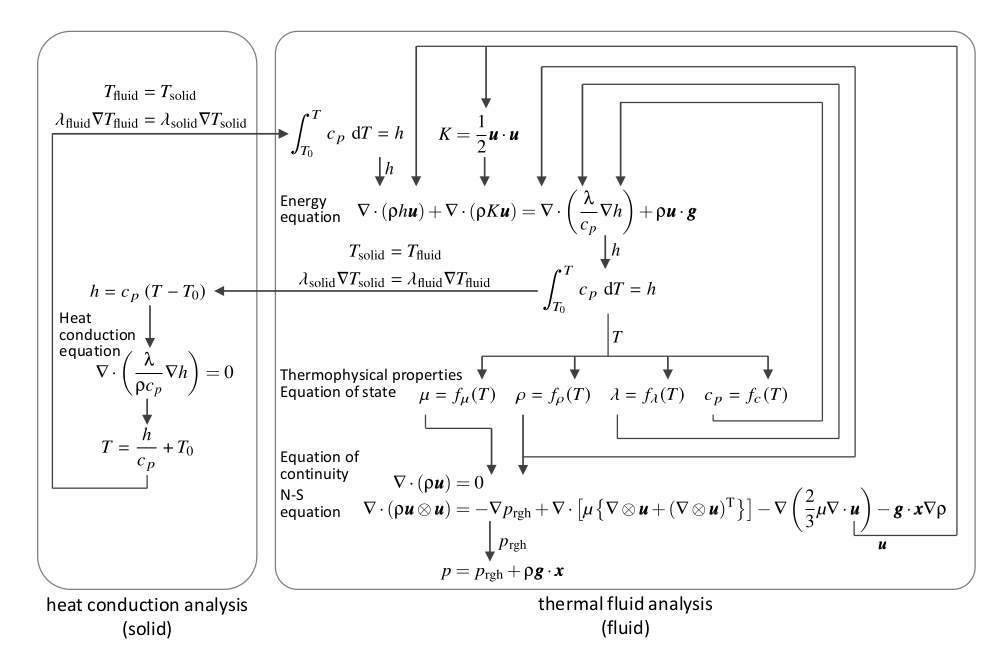
\includegraphics[width=\linewidth]{CHT_flowchart.png}	
	\label{4.2fig}
	\caption{Flowchart of the conjugate heat transfer solver \cite{sugimoto_kuramae_matsumoto_watanabe_2021}.}
\end{figure} 
\subsection{Code implementations}

\setlength{\parindent}{0.5cm} As remarked in the previous section, in the context of multiregion solvers, OpenFOAM offers the possibility of solving a fluid representing the compressible Navier-Stokes equations. However, the purpose of this final part is to enhance the capability of this solver so it can handle multiphase fluids submitted to conjugate heat transfer conditions.

\noindent To do so, and in favour of using the majority of possibilities that the solver brings, the energy equation in the solid part is kept without change. On the other side, the fluid part of the solver is implemented by integrating the multiphase solver used in the solidification section of this thesis.  

\noindent The implemented solver can be found in Appendix \ref{AppendixB} but here are presented the main changes.

\noindent The first change is the way in which the fluid is solved. In Fig. \ref{4.3fig} the loop in the fluid is corrected in such a way it incorporates the \textit{IcoReactingMultiphaseInterFoam} solver. 

\begin{figure}[h!]
	\centering
	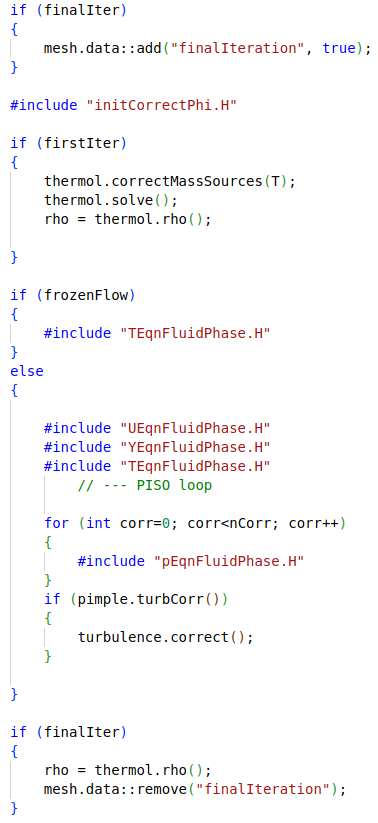
\includegraphics[width=0.4\linewidth]{fluid_loop.png}	
	\caption{Control loop for the fluid region in CHT.}
	\label{4.3fig}
\end{figure} 

\noindent On the other side, the energy equation is adapted so it can cope with multiphase fluids in the scope of multi region solvers. In the way of building up the equation, some of the terms that are newly introduced are the buoyancy energy, $\rho(U\&g)$, and the pressure terms $\nabla \cdot (\textbf{u}p)$ and the viscous dissipation term, $\nabla \cdot (\boldsymbol{\tau} \cdot \textbf{u})$, where $\tau$, the viscous stress tensor is calculated in the upper part of the code as the product of 2 by both the dynamic viscosity and the strain rate tensor.
\begin{equation}
\boldsymbol{\tau}=2 \mu \mathbf{D}
\end{equation}
Where \textbf{D} is the strain rate tensor:
\begin{equation}
	\mathbf{D}=-\frac{1}{2}\left[\nabla \mathbf{u}+\nabla \mathbf{u}^{\top}\right]=-\frac{1}{2}\left(\begin{array}{ccc}
	2 \frac{\partial u_{x}}{\partial x} & \frac{\partial u_{y}}{\partial x}+\frac{\partial u_{x}}{\partial y} & \frac{\partial u_{z}}{\partial x}+\frac{\partial u_{x}}{\partial z} \\
	\frac{\partial u_{x}}{\partial y}+\frac{\partial u_{y}}{\partial x} & 2 \frac{\partial u_{y}}{\partial y} & \frac{\partial u_{z}}{\partial y}+\frac{\partial u_{y}}{\partial z} \\
	\frac{\partial u_{x}}{\partial z}+\frac{\partial u_{z}}{\partial x} & \frac{\partial u_{y}}{\partial z}+\frac{\partial u_{z}}{\partial y} & 2 \frac{\partial u_{z}}{\partial z}
	\end{array}\right)
	\label{4.7}
\end{equation}
If substituting terms, it yields:
\begin{equation}
	\boldsymbol{\tau}=-\mu\left[\nabla \mathbf{u}+\nabla \mathbf{u}^{\top}\right]
	\label{4.8}
\end{equation}
\begin{figure}[h!]
	\centering
	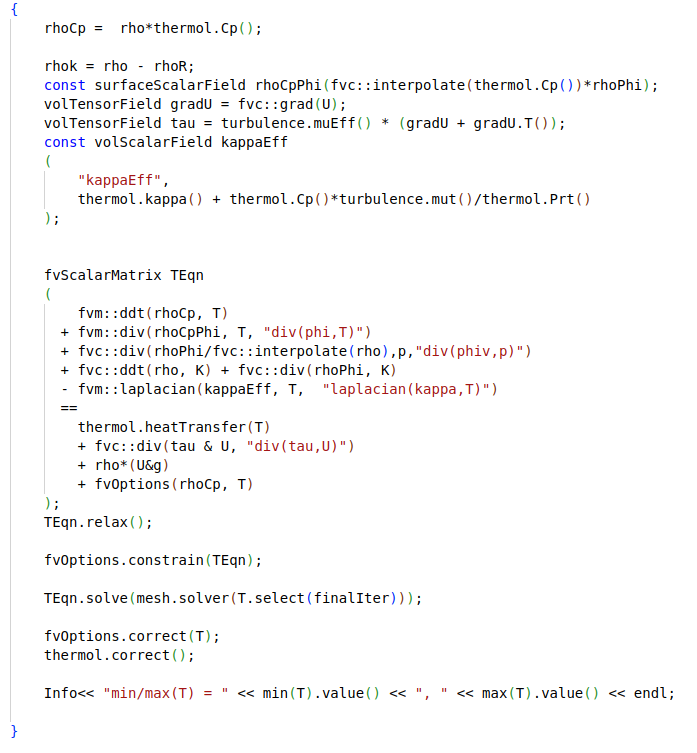
\includegraphics[width=0.9\linewidth]{TEqn_CHT.png}	
	\label{4.4fig}
	\caption{Energy equation for the fluid in CHT.}
\end{figure} 
\subsection{Case Setup}

\setlength{\parindent}{0.5cm} The case geometry is a plane cylinder, taking profit form the fluid mesh generated for the solidification case presented in the previous section. However, in this section, symmetry conditions are applied on the vertical axis (axis Y) so as to reduce the computational cost. 

\subsubsection{Boundary conditions}

\setlength{\parindent}{0.5cm} The boundary conditions are, in this case, setted up for both solid and fluid regions. Here it is shown a table summarizing the used ones.
\newline
For the fluid region:
\begin{table}[h!]
	\begin{tabular}{@{}lllll@{}}
		\toprule[1pt]
		\textbf{Boundary} & \textbf{Conditions}  \\ \midrule[2pt]
		Internal field & $ T = 298, u = 0, \alpha_{l} = 1, \alpha_{s} = 0    $  \\
		fluidFrontAndBack & empty \\
		fluidSymmetryBC & symmetryPlane \\ \bottomrule[1pt]		
	\end{tabular}
	\centering
	\caption{Boundary conditions for the fluid region in CHT problem.}	
	\label{4.1tab}
\end{table}
For the solid region:
\begin{table}[h!]
	\begin{tabular}{@{}lllll@{}}
		\toprule[1pt]
		\textbf{Boundary} & \textbf{Conditions}  \\ \midrule[2pt]
		Internal field & $ T = 298$\\
		solidWalls & $T = 258$ \\
		solidSymmetryBC & symmetryPlane \\
		solidFrontAndBack & empty \\ \bottomrule[1pt]		
	\end{tabular}
	\centering
	\caption{Boundary conditions for the solid region in CHT problem.}	
	\label{4.2tab}
\end{table}

\noindent At the interface between solid and liquid regions, it is required to set an appropriate boundary condition which couples the energy equations in these areas.

\noindent Considering two cells at each side of an interface in where $T_c$ and $T_p$ is the temperature at the cell center and on the patch (2D boundary) accordingly. $q_1$ is the heat flux going out of the $cell_1$ and $q_2$ the heat flux entering the $cell_2$. The energy conservation in this zone constrains the temperature and heat fluxes to be equat at both sides of the interface. 
Then, temperature, in magnitude yields as
\begin{equation}
	T_{p, 1}=T_{p, 2}=T_{p},
	\label{4.9}
\end{equation}
and as well, for the fluxes
\begin{equation}
	q_{1}^{\prime \prime}=q_{2}^{\prime \prime}=q^{\prime \prime}
	\label{4.10}
\end{equation}
while the magnitude for the heat fluxes is derived from the one-dimensional expression for the Fourier's law and it gives
\begin{equation}
	-\left.k_{1} \frac{\partial T}{\partial n}\right|_{\text {side } 1}=-\left.k_{2} \frac{\partial T}{\partial n}\right|_{\text {side } 2}
	\label{4.11}
\end{equation}
where $\kappa$ is the termal conductivity and $n$ the direction normal to the patch.

\noindent Discretizing linearly the temperature gradient of the previous equation, and with respect of the scheme of the Figure [], the differential equation that yields 
\begin{equation}
	k_{1} \Delta_{1}\left(T_{c, 1}-T_{p}\right)=k_{2} \Delta_{2}\left(T_{p}-T_{c, 2}\right)
	\label{4.12}
\end{equation}
where the temperatures and fluxes at the center of the patches are described as
\begin{equation}
	\begin{gathered}
	T_{p}=\frac{k_{1} \Delta_{1} T_{c, 1}+k_{2} \Delta_{2} T_{c, 2}}{k_{1} \Delta_{1}+k_{2} \Delta_{2}} \\
	q^{\prime \prime}=k_{1} \Delta_{1}\left(T_{c, 1}-T_{p}\right)=k_{2} \Delta_{2}\left(T_{p}-T_{c, 2}\right) .
	\end{gathered}
	\label{4.13}
\end{equation}
This boundary condition is given in OpenFOAM under the name \textit{turbulentTemperatureCoupledBaffleMixed}. The required input is the temperature at the patch. Therefore, that temperature for the interface between the liquid and the solid regions is initially setted at 298ºC.

\subsubsection{Thermophysical properties}

\setlength{\parindent}{0.5cm} The thermophysical properties for the fluid are similarly applied as in previous solidification cases.
For the solid region, the thermophysical properties are chosen as for the polyethylene.

\begin{table}[h!]
	\begin{tabular}{@{}lllll@{}}
		\toprule[1pt]
		\textbf{Polyethylene properties} & \textbf{Symbol} & \textbf{Values} & \textbf{Units} &  \\ \midrule[2pt]
		Density & $\rho$ & 940 & $kg.m^{-3}$ \\	
		Thermal conductivity & $\lambda$ & 0.56 & $W.m^{-1}.K^{-1}$ \\		
		Heat capacity & $C_{p}$ & 1330 & $J.kg.K^{-1}$ \\		 
		Latent heat & $L$ &  178600  & $J.K^{-1}$ \\		 \bottomrule[1pt]		
	\end{tabular}
	\centering
	\caption{Polyethylene properties for solind region definition.}	
	\label{4.3tab}
\end{table}

\subsection{Validation of Results and Conclusions}
\begin{table}[h!]
	\begin{tabular}{@{}llllll@{}}
		\toprule[1pt]
		 \multicolumn{1}{c}{\textbf{T}}& &\multicolumn{1}{c}{\textbf{U}}&
		 &\multicolumn{1}{c}{\textbf{$\alpha_{l}$}} & \\ \midrule[1pt]
		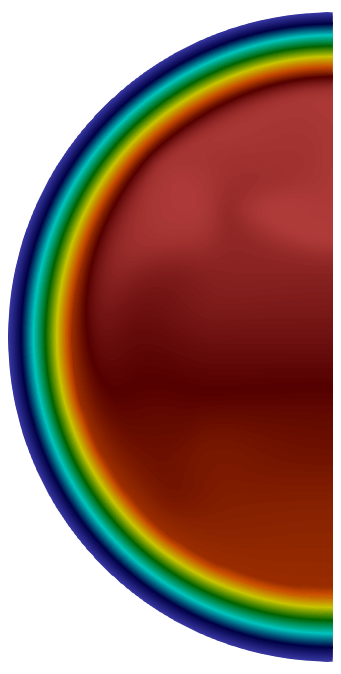
\includegraphics[width=0.21\linewidth]{T_CHT_NATIVE.png} & 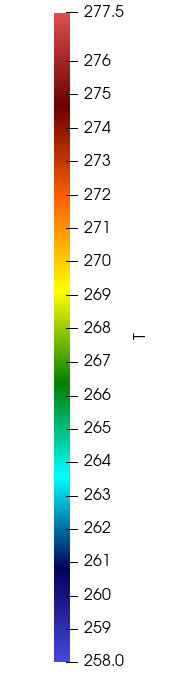
\includegraphics[width=.1\linewidth]{T_2100s_scale_EP_CHT.png} &
		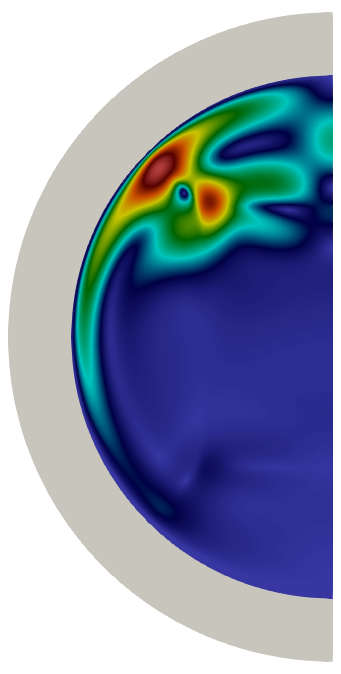
\includegraphics[width=0.21\linewidth]{U_CHT_NATIVE.png} & 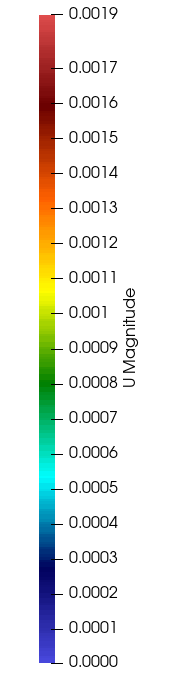
\includegraphics[width=.1\linewidth]{U_2100s_scale_EP_CHT.png} & 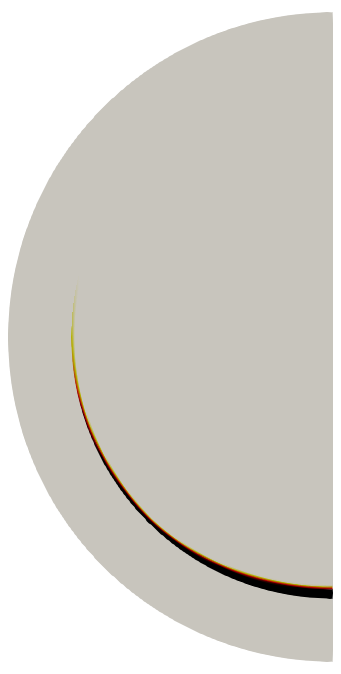
\includegraphics[width=0.21\linewidth]{ALPHA_CHT_NATIVE.png} & 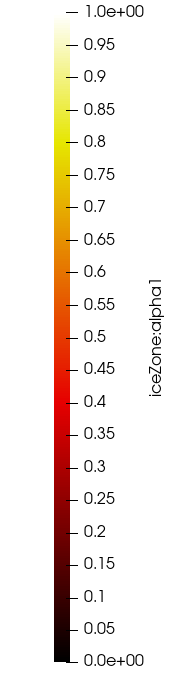
\includegraphics[width=.1\linewidth]{alpha_2100s_scale_EP_CHT.png}\\
		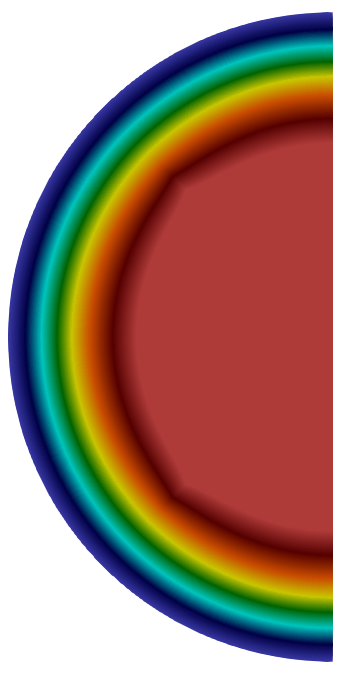
\includegraphics[width=0.21\linewidth]{T_CHT} & 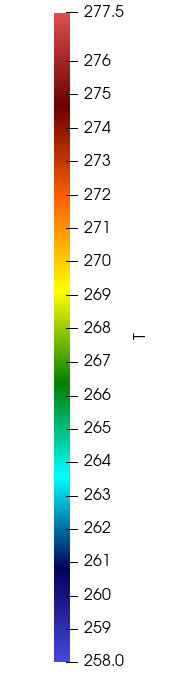
\includegraphics[width=.1\linewidth]{T_2100s_scale_EP_CHT.png} &
		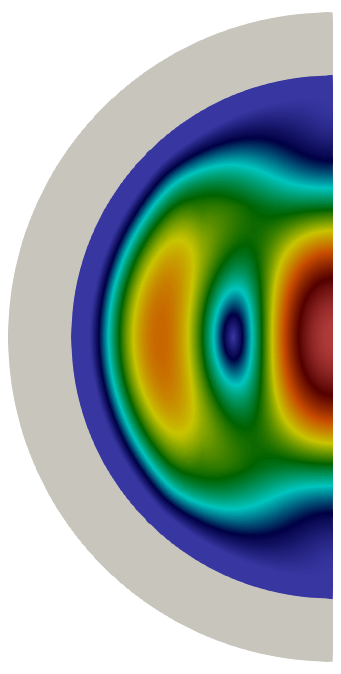
\includegraphics[width=0.21\linewidth]{U_CHT} & 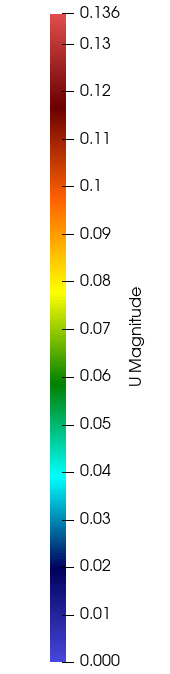
\includegraphics[width=.1\linewidth]{U_scale_CHT.png} & 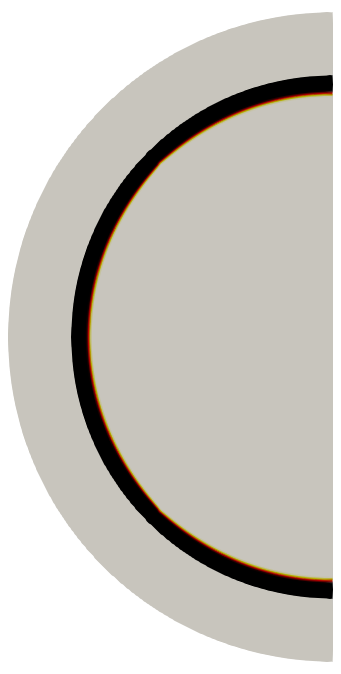
\includegraphics[width=0.21\linewidth]{alpha_CHT} & 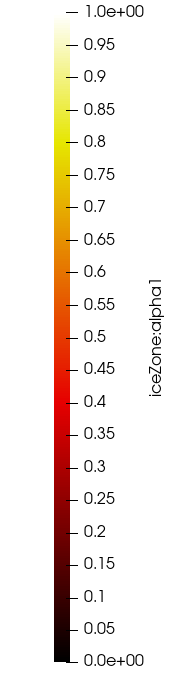
\includegraphics[width=0.1\linewidth]{alpha_2100s_scale_EP_CHT.png}\\ \bottomrule[1pt]		
	\end{tabular}
	\centering
	\caption{Numerical results of chtMultiRegionFoam (first row) and chtMultiPhaseInterFoam (second row) at \textit{t = 2100s} in a cylinder.}	
	\label{4.4tab}
\end{table}
